% ============================================================
% M2 轮4 S3 · 练习件 第7课时（§1.2.2 空间中的平面与空间向量）
% 题面：照题面库 成卷/题面库/课时07-1.2.2.md 全 16 题冻结入卷（卷面题号＝库序 1~16）；
%       组名/难度照库头第 3/4 字段（组名批替换后正名照录，去〔代表〕〔第2题〕簿记标）。
%       第4题库面「(多选)」随 \duoxuan 栏目标记承载（批1 课时03#3 先例），题面不再重复。
%       第13题「点M在线段BC上点M异于点B，C」＝源文（_tmp结构-讲上.json 1.2.2.6.1-7 行）原样，
%       疑脱括号→照录不改，登记待清稿轮。
%       第14题难度库标「中偏上→难档启用」→卷面印「难」（定稿B 升档口径），登记。
%       下标归一：库面 n2/u2/v2（抽取丢下标）→ n₂/u₂/v₂（同课时06 v2→v₂ 口径）。
% 图源（10 张，全部 figs/ 源位图，三维禁绘）：
%   #9  dy6_image22.png 30mm（单元6 image22·直三棱柱）
%   #10 dy3_image6.png  38mm（单元3 image6·正方体）
%   #11 js_image40.png  34mm（讲上 image40·正方体 E、F 中点）
%   #12 js_image42.png  34mm（讲上 image42·四棱锥 P-ABCD）
%   #13 js_image51.png 26mm＋js_image52.png 26mm（讲上双图行·截面四边形/临界）
%   #14 js_image50.png 22mm＋js_image48.png 24mm（讲上双图行·置①前）；js_image49.png 24mm（置①行后，源元素 542/543/545 结构）
%   #15 dy2_image14.png 30mm（单元2 image14·四棱锥 P-ABCD）
%   #16 复习题C·5 教材「如图所示」而库无【图】＝S1 冻结态、题面自足→不裁教材图，登记（同课时06#9/#16 口径）；
%       【装配轮0912】已删#16「如图所示，」语销债（题面自足、删语后无悬空指代；同拓册批6先例）。
% 【清稿注】三件（#10 DB∩DM=M→D、#11 补两平面不重合完备句、#14 ④维持相似比口径）＝答案册轮执行，
%   练习件卷面不印；#16 九字段亲算债（B-10）随台账续办。
% 取值/组名照登对照/图位/登记事项：见 ../批2值台账.md 课时07 节。
% 编译：xelatex main.tex（两遍）→ python render.py → png/pageN.png
% ============================================================
\documentclass[fontset=none]{ctexart}
\usepackage{qp-m3} % 换装：六宏→qp-m3 单包（钉后版 md5 7c3930362be8a0a2bdf21bbf8ac16573，两补钉随版）

% ============================================================
% 练习件局部宏（照练习线样张页2形制搬入；本段只加件，不改件）
% ============================================================
\renewcommand{\qpjianming}{练习件}
\renewcommand{\qpceming}{高中数学\quad 选择性必修第一册(人教B版)} % 换装回钉：qp-m3 默认册名＝选必二，防页脚漂移（试迁规约·试迁报告§四 B3 实证必改）
\renewcommand{\qpzhangming}{第一章\quad 空间向量与立体几何}

% ---------- YJ-01 灰块页脚·练习册档（块 31.0×7.8mm，照练习线样张 31.0mm 修正版） ----------
\newcommand{\qpxsyema}{\ifnum\value{page}<10 00\fi\ifnum\value{page}>9 \ifnum\value{page}<100 0\fi\fi\arabic{page}}
\newcommand{\lxshuziL}{\hbox to 13.8mm{\setlength{\fboxsep}{0pt}\colorbox{pnumbg}{%
  \makebox[31.0mm][l]{\rule[-3.145mm]{0pt}{7.8mm}\hspace{2.8mm}\fontsize{10.7pt}{13pt}\selectfont\color{black}\numpnum\qpxsyema}}\hss}}
\newcommand{\lxshuziR}{\hbox to 13.8mm{\kern-17.2mm\setlength{\fboxsep}{0pt}\colorbox{pnumbg}{%
  \makebox[31.0mm][r]{\rule[-3.145mm]{0pt}{7.8mm}\fontsize{10.7pt}{13pt}\selectfont\color{black}\numpnum\qpxsyema\hspace{2.75mm}}}}}
\fancyfoot[RO]{\raisebox{-1.24mm}[0pt][0pt]{\qphuitext\qpzhangming\quad{\heiti\qpjianming}\hspace{3mm}\lxshuziL}}
\fancyfoot[LE]{\raisebox{-1.24mm}[0pt][0pt]{\lxshuziR\hspace{3mm}\qphuitext\qpceming}}

% ---------- HX-01 花形·三档名（练习册版 25.5×6.8mm，重叠 o＝5.1mm，照练习线样张裁定值） ----------
% 局部宏 \huadianOverlapLx 已由 qp-m3 收编（等值定义），依换装方案§1.4 预删防撞名
% 局部宏 \dangbadge 已由 qp-m3 收编（等值定义），依换装方案§1.4 预删防撞名

% ---------- TJ-02 练习册悬挂题号（单号 5.75mm／双位 7.6mm，题号 \textbf 加重） ----------
% 长度 \lxhang 已由 qp-m3 分配，预删防重复定义
% 局部宏 \tihao 已由 qp-m3 收编（等值定义），依换装方案§1.4 预删防撞名
% 选项段（TJ-07 行距档；左缘随题号悬挂）
% 局部宏 \lxopt 已由 qp-m3 收编（等值定义），依换装方案§1.4 预删防撞名
% 解答题书写位留白
% 局部宏 \xiexwei 已由 qp-m3 收编（等值定义），依换装方案§1.4 预删防撞名
% 组名栏宏（组名照题面库头第 3 字段照登，去〔代表〕〔第N题〕簿记标）
% 局部宏 \zu 已由 qp-m3 收编（等值定义），依换装方案§1.4 预删防撞名

\begin{document}

% ============================================================
% 课时训练（三档 10＋4＋2＝16 题）
% ============================================================
\keshi{第7课时\quad 空间中的平面与空间向量}
\begin{multicols}{2}
\emergencystretch=1em

\dangbadge{基}{础}{巩}{固}

\tihao{1}\zu{K1 平面的法向量·求法（方程组法）} \tieside{简单}若两个向量\(\overrightarrow{AB}=(1,2,3)\)，\(\overrightarrow{AC}=(3,2,1)\)，则平面\(ABC\)的一个法向量为\nobreak(\kongwei)
\lxopt{\makebox[\dimexpr0.5\linewidth-0.5\lxhang-0.25em\relax][l]{A．\((-1,2,-1)\)；}\makebox[\dimexpr0.5\linewidth-0.5\lxhang-0.25em\relax][l]{B．\((1,2,1)\)}}
\lxopt{\makebox[\dimexpr0.5\linewidth-0.5\lxhang-0.25em\relax][l]{C．\((1,2,-1)\)；}\makebox[\dimexpr0.5\linewidth-0.5\lxhang-0.25em\relax][l]{D．\((-1,2,1)\)}}
\begin{ansblock}[练-课时07-1]
% ans:练-课时07-1
\ansitem{1}{A\((-1,2,-1)\)}
\end{ansblock}

\tihao{2}\zu{K2 法向量性质·点面归属判定} \tieside{简单}已知平面\(\alpha\)内有一点\(M(1,-1,2)\)，平面\(\alpha\)的一个法向量为\(\overrightarrow{n}=(6,-3,6)\)，则下列点\(P\)中，在平面\(\alpha\)内的是\nobreak(\kongwei)
\lxopt{\makebox[\dimexpr0.5\linewidth-0.5\lxhang-0.25em\relax][l]{A．\(P(2,3,3)\)；}\makebox[\dimexpr0.5\linewidth-0.5\lxhang-0.25em\relax][l]{B．\(P(-2,0,1)\)}}
\lxopt{\makebox[\dimexpr0.5\linewidth-0.5\lxhang-0.25em\relax][l]{C．\(P(-4,4,0)\)；}\makebox[\dimexpr0.5\linewidth-0.5\lxhang-0.25em\relax][l]{D．\(P(3,-3,4)\)}}
\begin{ansblock}[练-课时07-2]
% ans:练-课时07-2
\ansitem{2}{A\((2,3,3)\)}
\end{ansblock}

\tihao{3}\zu{K3 线面位置关系·法向量判定选型} \tieside{简单}已知直线\(l\)的方向向量是\(\overrightarrow{a}=(3,2,1)\)，平面\(\alpha\)的法向量是\(\overrightarrow{u}=(-1,2,-1)\)，则\(l\)与\(\alpha\)的位置关系是\nobreak(\kongwei)
\lxopt{\makebox[\dimexpr0.5\linewidth-0.5\lxhang-0.25em\relax][l]{A．\(l\perp\alpha\)；}\makebox[\dimexpr0.5\linewidth-0.5\lxhang-0.25em\relax][l]{B．\(l\parallel\alpha\)}}
\lxopt{C．\(l\)与\(\alpha\)相交但不垂直；}
\lxopt{D．\(l\parallel\alpha\)或\(l\subset\alpha\)．}
\begin{ansblock}[练-课时07-3]
% ans:练-课时07-3
\ansitem{3}{D}
\end{ansblock}

\tihao{4}\duoxuan\zu{K3 四命题多选集中辨析} \tieside{简单}下列命题是真命题的有\nobreak(\kongwei)．
\lxopt{A．直线\(l\)的方向向量为\(\overrightarrow{a}=(1,-1,2)\)，直线\(m\)的方向向量为\(\overrightarrow{b}=(2,1,-\frac{1}{2})\)，则\(l\)与\(m\)垂直}
\lxopt{B．直线\(l\)的方向向量为\(\overrightarrow{a}=(0,1,-1)\)，平面\(\alpha\)的法向量为\(\overrightarrow{n}=(1,-1,-1)\)，则\(l\perp\alpha\)}
\lxopt{C．平面\(\alpha\)，\(\beta\)的法向量分别为\(\overrightarrow{n_1}=(0,1,3)\)，\(\overrightarrow{n_2}=(1,0,2)\)，则\(\alpha\parallel\beta\)}
\lxopt{D．平面\(\alpha\)经过三点\(A(1,0,-1)\)，\(B(0,1,0)\)，\(C(-1,2,0)\)，向量\(\overrightarrow{n}=(1,u,t)\)是平面\(\alpha\)的法向量，则\(u+t=1\)}
\begin{ansblock}[练-课时07-4]
% ans:练-课时07-4
\ansitem{4}{AD}
\end{ansblock}

\tihao{5}\zu{K4 法向量判面面平行·共线条件} \tieside{简单}平面\(\alpha\)的一个法向量为\(\overrightarrow{v_1}=(1,2,1)\)，平面\(\beta\)的一个法向量\(\overrightarrow{v_2}=-(2,4,2)\)，则平面\(\alpha\)与平面\(\beta\)\nobreak(\kongwei)
\lxopt{\makebox[\dimexpr0.5\linewidth-0.5\lxhang-0.25em\relax][l]{A．平行；}\makebox[\dimexpr0.5\linewidth-0.5\lxhang-0.25em\relax][l]{B．垂直}}
\lxopt{\makebox[\dimexpr0.5\linewidth-0.5\lxhang-0.25em\relax][l]{C．相交；}\makebox[\dimexpr0.5\linewidth-0.5\lxhang-0.25em\relax][l]{D．不能确定}}
\begin{ansblock}[练-课时07-5]
% ans:练-课时07-5
\ansitem{5}{A（平行）}
\end{ansblock}

\tihao{6}\zu{K4 求出法向量后逐对判多位置} \tieside{简单}设\(\overrightarrow{n_1}\)，\(\overrightarrow{n_2}\)分别是空间中两个不重合的平面\(\alpha\)，\(\beta\)的法向量，分别根据下列条件判断平面\(\alpha\)，\(\beta\)的位置关系：
\lxopt{(1)\(\overrightarrow{n_1}=(-2,1,2)\)，\(\overrightarrow{n_2}=(6,-3,-6)\)；}
\lxopt{(2)\(\overrightarrow{n_1}=(1,2,3)\)，\(\overrightarrow{n_2}=(3,6,9)\)．}
\xiexwei{16mm}
\begin{ansblock}[练-课时07-6]
% ans:练-课时07-6
\ansitem{6}{(1)(2) 均 \(\alpha\parallel\beta\)}
\end{ansblock}

\tihao{7}\zu{K5 法向量判面面垂直·点积为零} \tieside{简单}设\(\overrightarrow{n_1}=(-2,2,5)\)，\(\overrightarrow{n_2}=(3,-2,2)\)分别是空间中平面\(\alpha\)，\(\beta\)的法向量，判断平面\(\alpha\)，\(\beta\)是否垂直．
\xiexwei{16mm}
\begin{ansblock}[练-课时07-7]
% ans:练-课时07-7
\ansitem{7}{垂直}
\end{ansblock}

\tihao{8}\zu{K6 法向量共线·反求参数} \tieside{简单}若平面\(\alpha\)的一个法向量为\(\overrightarrow{u_1}=(-3,y,2)\)，平面\(\beta\)的一个法向量为\(\overrightarrow{u_2}=(6,-2,z)\)，且\(\alpha\parallel\beta\)，则\(y+z=\)\kongbai{}．
\begin{ansblock}[练-课时07-8]
% ans:练-课时07-8
\ansitem{8}{\(-3\)}
\end{ansblock}

\tihao{9}\zu{K7 线面平行·开放条件补全} \tieside{简单}在直三棱柱\(ABC\text{-}\penalty100 A_1B_1C_1\)中，\(D\)为\(AA_1\)中点，点\(P\)在侧面\(BCC_1B_1\)上运动，当点\(P\)满足条件\kongbai{}时，\(A_1P\parallel\)平面\(BCD\)（答案不唯一，填一个满足题意的条件即可）．
\par\vspace{1.9mm}\penalty10000\noindent\makebox[\linewidth][c]{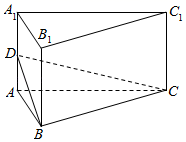
\includegraphics[width=30mm]{figs/dy6_image22.png}}\par\vspace{-1.0mm}\penalty-50
\begin{ansblock}[练-课时07-9]
% ans:练-课时07-9
\ansitem{9}{\(P\) 为 \(CC_{1}\) 中点（答案不唯一）}
\end{ansblock}

\tihao{10}\zu{K8 线面垂直·坐标法证明（正方体构形）} \tieside{简单}如图，在正方体\(ABCD\text{-}\penalty100 A_1B_1C_1D_1\)中，\(O\)是\(AC\)与\(BD\)的交点，\(M\)是\(CC_1\)的中点．求证：\(A_1O\perp\)平面\(MBD\)．
\par\vspace{1.9mm}\penalty10000\noindent\makebox[\linewidth][c]{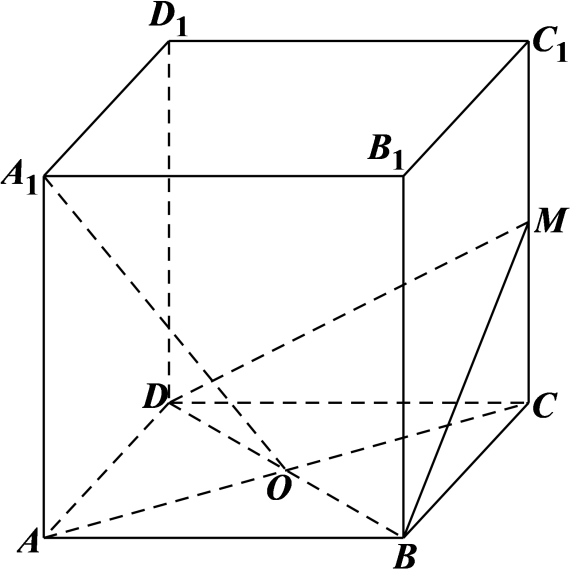
\includegraphics[width=38mm]{figs/dy3_image6.png}}\par\vspace{-1.0mm}\penalty-50
\xiexwei{16mm}
\begin{ansblock}[练-课时07-10]
% ans:练-课时07-10
\setlength{\anshang}{7.6mm}% 题10 起双位档（照答案册同值，块内局部）
\ansitem{10}{证明见解析}
\ansnote{解析}{末句 \(DB\cap DM=D\)。}
\end{ansblock}

\dangbadge{综}{合}{提}{升}

\tihao{11}\zu{K9 线面平行＋面面平行·法向量判定证明（双判据门面）} \tieside{中档}已知正方体\(ABCD\text{-}\penalty100 A_1B_1C_1D_1\)的棱长为\(2\)，\(E\)，\(F\)分别是\(BB_1\)，\(DD_1\)的中点，
\par\vspace{1.9mm}\penalty10000\noindent\makebox[\linewidth][c]{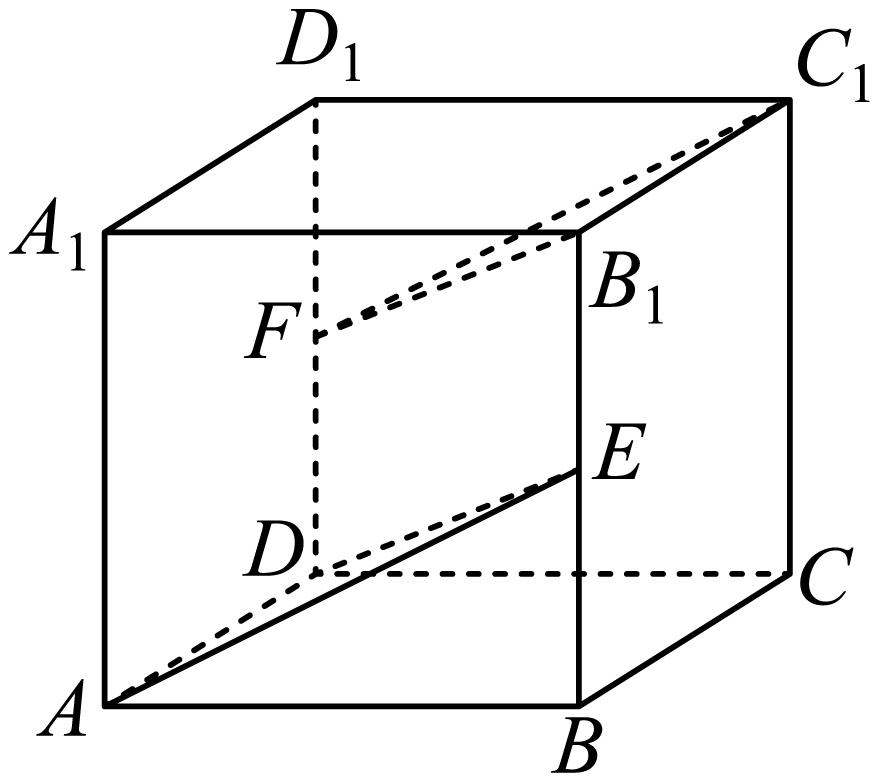
\includegraphics[width=34mm]{figs/js_image40.png}}\par\vspace{-1.0mm}\penalty10000
\lxopt{求证：(1)\(FC_1\parallel\)平面\(ADE\)；(2)平面\(ADE\parallel\)平面\(B_1C_1F\)．}
\xiexwei{16mm}
\begin{ansblock}[练-课时07-11]
% ans:练-课时07-11
\setlength{\anshang}{7.6mm}% 题11 起双位档（照答案册同值，块内局部）
\ansitem{11}{(1)(2) 证明见解析}
\ansnote{解析}{法向量共线 \(\Rightarrow\) 平行或重合；又两平面不重合，故平行。}
\end{ansblock}

\tihao{12}\zu{K10 垂直/平行存在性·含参双问} \tieside{中档}如图所示，在四棱锥\(P\text{-}\penalty100 ABCD\)中，底面\(ABCD\)为正方形，\(PA\perp\)平面\(ABCD\)，点\(E\)在线段\(PC\)上（不含端点）．
\par\vspace{1.9mm}\penalty10000\noindent\makebox[\linewidth][c]{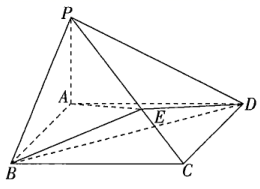
\includegraphics[width=34mm]{figs/js_image42.png}}\par\vspace{-1.0mm}\penalty10000
\lxopt{(1)是否存在点\(E\)，使\(PC\perp\)平面\(BDE\)？}
\lxopt{(2)是否存在点\(E\)，使平面\(PCD\perp\)平面\(AED\)？}
\xiexwei{16mm}
\begin{ansblock}[练-课时07-12]
% ans:练-课时07-12
\setlength{\anshang}{7.6mm}% 题12 起双位档（照答案册同值，块内局部）
\ansitem{12}{(1)存在，\(PE=\dfrac{a^{2}+c^{2}}{2a^{2}+c^{2}}PC\)；(2)不存在}
\end{ansblock}

\tihao{13}\zu{K11 截面·形状临界定范围} \tieside{中档}已知正方体\(ABCD\text{-}\penalty100 A_1B_1C_1D_1\)的体积为\(1\)，点\(M\)在线段\(BC\)上点\(M\)异于点\(B\)，\(C\)，点\(N\)在线段\(CC_1\)上，且\(CN=\frac{1}{3}\)，若平面\(AMN\)截正方体\(ABCD\text{-}\penalty100 A_1B_1C_1D_1\)所得的截面为四边形，则线段\(BM\)长的取值范围为\nobreak(\kongwei)
\par\vspace{1.9mm}\penalty10000\noindent\makebox[\linewidth][c]{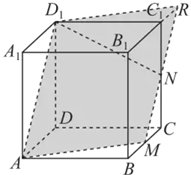
\includegraphics[width=26mm]{figs/js_image51.png}\hspace{4mm}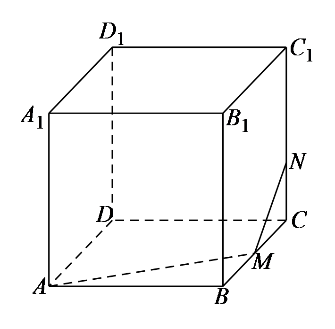
\includegraphics[width=26mm]{figs/js_image52.png}}\par\vspace{-1.0mm}\penalty10000
\lxopt{\makebox[\dimexpr0.5\linewidth-0.5\lxhang-0.25em\relax][l]{A．\([\frac{2}{3},1)\)；}\makebox[\dimexpr0.5\linewidth-0.5\lxhang-0.25em\relax][l]{B．\([\frac{1}{3},\frac{2}{3}]\)}}
\lxopt{\makebox[\dimexpr0.5\linewidth-0.5\lxhang-0.25em\relax][l]{C．\((0,\frac{1}{3}]\)；}\makebox[\dimexpr0.5\linewidth-0.5\lxhang-0.25em\relax][l]{D．\((0,\frac{2}{3}]\)}}
\begin{ansblock}[练-课时07-13]
% ans:练-课时07-13
\setlength{\anshang}{7.6mm}% 题13 起双位档（照答案册同值，块内局部）
\ansitem{13}{D（\(\left(0,\dfrac{2}{3}\right]\)）}
\end{ansblock}

\tihao{14}\zu{K12 截面·多说法复合判定（大招6 讲例绑定）} \tieside{难}如图，四棱柱\(ABCD\text{-}\penalty100 A_1B_1C_1D_1\)的底面是边长为\(2\)的正方形，侧棱\(AA_1\perp\)平面\(ABCD\)，且\(AA_1=4\)，\(E\)、\(F\)分别是\(AB\)、\(BC\)的中点，\(P\)是线段\(DD_1\)上的一个动点（不含端点），过\(P\)、\(E\)、\(F\)的平面记为\(\alpha\)，\(Q\)在\(CC_1\)上且\(CQ=1\)，则下列说法正确的个数是\nobreak(\kongwei)．
\par\vspace{1.9mm}\penalty10000\noindent\makebox[\linewidth][c]{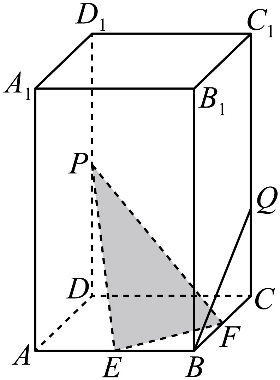
\includegraphics[width=22mm]{figs/js_image50.png}\hspace{4mm}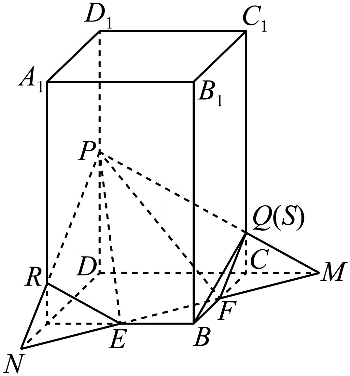
\includegraphics[width=24mm]{figs/js_image48.png}}\par\vspace{-1.0mm}\penalty10000
\lxopt{①三棱锥\(C_1\text{-}\penalty100 PAC\)的体积是定值；}
\par\vspace{1.9mm}\penalty10000\noindent\makebox[\linewidth][c]{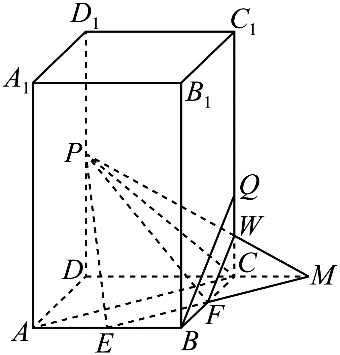
\includegraphics[width=24mm]{figs/js_image49.png}}\par\vspace{-1.0mm}\penalty10000
\lxopt{②当直线\(BQ\parallel\alpha\)时，\(DP=2\)；③当\(DP=3\)时，平面\(\alpha\)截棱柱所得多边形的周长为\(7\sqrt{2}\)；④存在平面\(\alpha\)，使得点\(A_1\)到平面\(\alpha\)距离是\(A\)到平面\(\alpha\)距离的两倍．}
\lxopt{\makebox[\dimexpr0.25\linewidth-0.25\lxhang-0.25em\relax][l]{A．\(1\)；}\makebox[\dimexpr0.25\linewidth-0.25\lxhang-0.25em\relax][l]{B．\(2\)；}\makebox[\dimexpr0.25\linewidth-0.25\lxhang-0.25em\relax][l]{C．\(3\)；}\makebox[\dimexpr0.25\linewidth-0.25\lxhang-0.25em\relax][l]{D．\(4\)}}
\begin{ansblock}[练-课时07-14]
% ans:练-课时07-14
\setlength{\anshang}{7.6mm}% 题14 起双位档（照答案册同值，块内局部）
\ansitem{14}{B（\(2\) 个）}
\ansnote{解析}{④按相似比讲解。}
\end{ansblock}

\dangbadge{思}{维}{探}{索}

\tihao{15}\zu{K13 线面垂直·数量积拆分证明} \tieside{中档}如图所示，在四棱锥\(P\text{-}\penalty100 ABCD\)中，\(PA\perp\)底面\(ABCD\)，\(AB\perp AD\)，\(AC\perp CD\)，\(\angle ABC=60^{\circ}\)，\(PA=AB=BC\)，\(E\)是\(PC\)的中点．证明：
\par\vspace{1.9mm}\penalty10000\noindent\makebox[\linewidth][c]{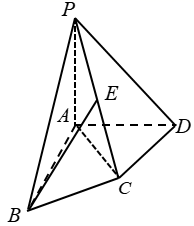
\includegraphics[width=30mm]{figs/dy2_image14.png}}\par\vspace{-1.0mm}\penalty10000
\lxopt{(1)\(CD\perp AE\)；}
\lxopt{(2)\(PD\perp\)平面\(ABE\)．}
\xiexwei{16mm}
\begin{ansblock}[练-课时07-15]
% ans:练-课时07-15
\setlength{\anshang}{7.6mm}% 题15 起双位档（照答案册同值，块内局部）
\ansitem{15}{(1)(2) 证明见解析}
\end{ansblock}

\tihao{16}\zu{K14 线线垂直证明＋体积（教材C组大题）} \tieside{难}在三棱锥\(P\text{-}\penalty100 ABC\)中，\(\triangle PAB\)是等边三角形，\(\angle PAC=\angle PBC=90^{\circ}\)．
\lxopt{(1)证明：\(AB\perp PC\)；}
\lxopt{(2)若\(PC=4\)，且平面\(PAC\perp\)平面\(PBC\)，求三棱锥\(P\text{-}\penalty100 ABC\)的体积．}
\xiexwei{20mm}
\begin{ansblock}[练-课时07-16]
% ans:练-课时07-16
\setlength{\anshang}{7.6mm}% 题16 起双位档（照答案册同值，块内局部）
\ansitem{16}{(1)证明见解析；(2)\(V=\dfrac{8}{3}\)}
\end{ansblock}

\end{multicols}

\tailfill
\end{document}
